\documentclass[12pt]{article}

% \usepackage{fullpage}
\usepackage{titling}
\usepackage{amsmath}
\usepackage{graphicx}
\usepackage{etoolbox}
\usepackage{pbox}
\usepackage{float}
\usepackage{sectsty}
\graphicspath{ {./resources/} }
\patchcmd{\thebibliography}{\section*{\refname}}{}{}{}

\sectionfont{\fontsize{14}{12}\selectfont}

\setlength{\droptitle}{-5em}

\setlength{\parindent}{0pt}
\addtolength{\oddsidemargin}{-1.2in}
\addtolength{\evensidemargin}{-1.2in}
\addtolength{\textwidth}{2.4in}

\addtolength{\topmargin}{-1.3in}
\addtolength{\textheight}{2.5in}

\title{CS3243 Tetris Project}
\author{}
\date{}

\begin{document}
	\vspace{-4cm}
	\pagenumbering{gobble}
	\maketitle
	\thispagestyle{empty}
	\vspace{-3cm}

	{\small Varun Gupta \;\;\;\;  Gao Bo \;\;\;\; Advay Pal \;\;\;\; Chang Chu-Ming \;\;\;\; Herbert Ilhan Tanujaya}\\
	{\small A0147924X \;\;\;\;  A0121585H \;\;\;\; Advay Pal \;\;\;\; Chang Chu-Ming \;\;\;\; Herbert Ilhan Tanujaya}

    \section{Introduction}
	\vspace{-0.3cm}
    In this report, we describe how we devise an agent to play the game of Tetris.
    We use an agent that greedily picks the best possible next state from a given state,
    by using a heuristic function to approximate the value of a state. To train our heuristic
    function, we use a novel algorithm that is a combination of a Genetic Algorithm (GA)
    and Particle Swarm Algorithm (PSO). Our agent manages to clear \textbf{TODO} million lines on average with a max
    of \textbf{TODO} million lines, demonstrating that our algorithm is effective.

	\vspace{-0.3cm}
    \section{Agent Strategy}
	\vspace{-0.3cm}
	Our agent uses a linear weighted sum of features as the heuristic function for
	a given state(configuration of the board). Given a
	state and a piece, the agent computes the heuristic value for all possible next
	states, and then greedily picks the next state with the maximum heuristic
	value. In other words, the next state is chosen by \small \[ \max_{s' \in N(s, p)}
	\left\{ \sum w_i f_i(s') \right\}, \] \normalsize where $s$ is the original state, $N(s,
	p)$ is the set of all possible next states from $s$ and a piece $p$, $f_i(s')$
	is the score of feature $i$ on state $s'$ and $w_i$ is the weight of feature
	$i$.

	\vspace{-0.3cm}
    \section{Features}
	\vspace{-0.3cm}
    We used the following features for our heuristic function:
    \begin{itemize}
		\setlength\itemsep{-1mm}
        \item \textbf{Altitude Difference} ($AltD$): Difference between height of the highest
        and the lowest column
		\item \textbf{Column Transition} ($ColT$): Number of adjacent squares in a column with opposite parity (where parity is defined as either full or empty)
		\item \textbf{Deepest Well} ($DW$): Height of the lowest column
        \item \textbf{Height} ($ColH$): Height of the highest column
		\item \textbf{Number of Columns With Holes} ($CwH$): The number of columns with holes, where a hole
		is defined as an empty square directly beneath a filled square
        \item \textbf{Number of Holes} ($NHole$): Number of holes in the entire board
        \item \textbf{Number of Wells} ($NWell$): Number of columns that have height less than the 2
        adjacent columns
		\item \textbf{Rows Cleared} ($RC$): Number of rows cleared for that particular move
		\item \textbf{Row Transition} ($RowT$): Number of adjacent squares in a row with opposite parity
        \item \textbf{Total Column Height} ($TColH$): The sum of the heights of all the columns
        \item \textbf{Total Column Height Difference} ($TColHD$): The sum of the difference of heights between adjacent columns
        \item \textbf{Weighted Block} ($WB$): Sum of value of every filled square, where a square's value is equal to
		the row it is in (numbered from the bottom)
        \item \textbf{Well Sum} ($WellS$): Sums up the depth of every well
    \end{itemize}

    % While running our training algorithms, we noticed that some features were more
	% important than others. In particular, the algorithm assigned highly negative
	% weights to Column Transition and Well Sum, while assigning highly positive
	% weights to Number of Wells. This was slightly unexpected as we thought that
	% Rows Cleared would have the largest positive weights, to predispose the algorithm
	% towards clearing more rows. However, the weight for this heuristic varied wildly
	% between positive and negative, indicating that perhaps sometimes the algorithm
	% preferred to not greedily pick moves that were clearing rows, choosing instead
	% to maintain an even surface at the top.

	\vspace{-0.3cm}
    \section{Our Algorithm}
	\vspace{-0.2cm}

    Our algorithm consists of a combination of a GA and PSO algorithm. We run both of these algorithms on different ‘islands’
	with population sizes of a 100 each. Each member of our population is a heuristic (set of weights).
	The key idea is that both of the algorithms run individually, but after each generation, we
	copy the 10 best heuristics on each island to the other one.\\

	\textbf{Genetic Algorithm} -
	We use a standard GA with crossover and mutation. A crossover is
	done by taking two parent heuristics, and,
	for every feature, selecting the weight from one of the parents randomly. A
	mutation is defined as multiplying the current weight of a feature with
	a value normally distributed with a mean of 1 and a standard deviation of 1. Parents are chosen based on fitness, with fitter population members having a higher
	probability of being chosen. We keep the top half of the population to ensure that each set of heuristics
	that perform well will remain within the population and replace the bottom half with
	new members.\\

	\textbf{PSO algorithm} -
	We use a standard PSO algorithm which treats every heuristic as a point in 13-dimensional space.
	This is the position of the heuristic. Each heuristic also has a velocity,
	a vector in the 13-dimensional space, which is added to the position to get
	new population members. New velocities are computed by taking a linear weighted
	sum of the old velocity, the personal best of that member, and the global best.\\

	\textbf{Rationale behind combination of algorithms} -
	We first ran PSO and GA individually. Doing so, we realised that while PSO didn't do too well
	it's fitness sometimes jumped by almost an order of magnitude.
	On the other hand, GA seemed to keep getting
	better, but only quite slowly. We hypothesised
	that GA may be doing more of exploitation, finding the maximum in the local area,
	while PSO may have been doing more of exploration, looking for good solutions all over
	the search space. We therefore decided to combine the two, as this
	would allow us to achieve a more balanced trade-off between exploitation
	and exploration, thereby improving efficiency.

	\vspace{-0.3cm}
	\section{Further Optimisation}
	\vspace{-0.2cm}
	The hyperparameters for both the GA and the PSO algorithm need
	to be optimized for our integrated solution to learn at an optimal rate.
	We decided to focus our attention on the hyperparameters
	of the PSO algorithm. Since PSO looked to be exploring the state space, successfully
	optimising it, might enable it to find a solution close to the global
	maximum and share this information with the GA which could then refine the solution further.\\

	The hyperparameters of the PSO algorithm consist of $\rho_g$ and $\rho_p$, the constants
	which determine the effect of the global and personal bests on each iteration
	of velocity change; and $\omega$, the constant of inertia. Typically \cite{alam2015comparative}, $\rho_g$ and $\rho_p$ are both
	set to 2.0[1], which leaves $\omega$ to be optimized. A high $\omega$ will favour exploration,
	while a low $\omega$ will favour exploitation. Based on the observations of
	\cite{shi1998parameter}, we decided to first test values of $\omega$ between 0.6 to 1.2.
	While initializations with low $\omega$ generally performed better, the results were
	not conclusive. Thus, we decided that instead of a fixed $\omega$, we could vary it
	based on how close the population is to the global maximum. This is estimated
	by taking $\log_{10}$ of the average fitness scores of the population. The formula is as follows:

	\begin{center}
		$\omega = 1.2 - k(\log_{10}\text{(Average Fitness)} - 3)$
	\end{center}

	We tested different values of $k$ by running multiple jobs for an hour and comparing
 	the average of the fitness scores. Through experimentation, we found that the
	algorithm performs best when $k$ is 0.2.\\

	% Note: The values below are taken across 5 instances with the same hyperparameters.\\

	% \twocolumn
	% \underline{Fixing and tuning $\omega$}\\
	% Lower $\omega$ = more exploitation, worse maximum, better average\\
	% Higher $\omega$ = more exploration, better maximum, worse average\\

	% \begin{tabular}{ | c | c | c | }
	% 	\hline
	% 	$\omega$ & \parbox{3cm}{\centering Maximum of \\Average Fitness} & \pbox{20cm}{Average of \\Average Fitness} \\[2ex] \hline
	% 	0.6 & 44807 & 30935 \\ \hline
	% 	0.8 & 58192 & 27357 \\ \hline
	% 	1.0 & 69375 & 26849 \\ \hline
	% 	1.2 & 72743 & 20381 \\ \hline
	% \end{tabular}

	% \underline{Varying $\omega$ and tuning $k$}\\
	% Higher $k$ = more varying $\omega$ = stronger transition from exploration to exploitation\\
	% Lower $k$ = less varying $\omega$ = weaker transition from exploration to exploitation\\
	%
	% \begin{tabular}{ | c | c | c c c | c | c | }
	% 	\hline
	% 	$k$ & \parbox{3cm}{\centering Maximum of \\Average Fitness} & \pbox{20cm}{Average of \\Average Fitness} & & $\omega$ & \parbox{3cm}{\centering Maximum of \\Average Fitness} & \pbox{20cm}{Average of \\Average Fitness} \\ \hline
	% 	0.1 & 50260 & 32939 & & 0.6 & 44807 & 30935 \\ \hline
	% 	0.15 & 47115 & 30010 & & 0.8 & 58192 & 27357 \\ \hline
	% 	0.2 & 74838 & 38478 & & 1.0 & 69375 & 26849\\ \hline
	% \end{tabular}

	% \onecolumn

	\vspace{-0.3cm}
    \section{Experiments and Analysis}

	\textbf{Learning Perfomance}\\
	We ran our learning algorithm on nodes provided by the National Supercomputing Centre cluster
	with specifications: E5-2690 v3 @ 2.60GHz.
	Using this, the results we obtained were:

	\begin{figure}[h]
		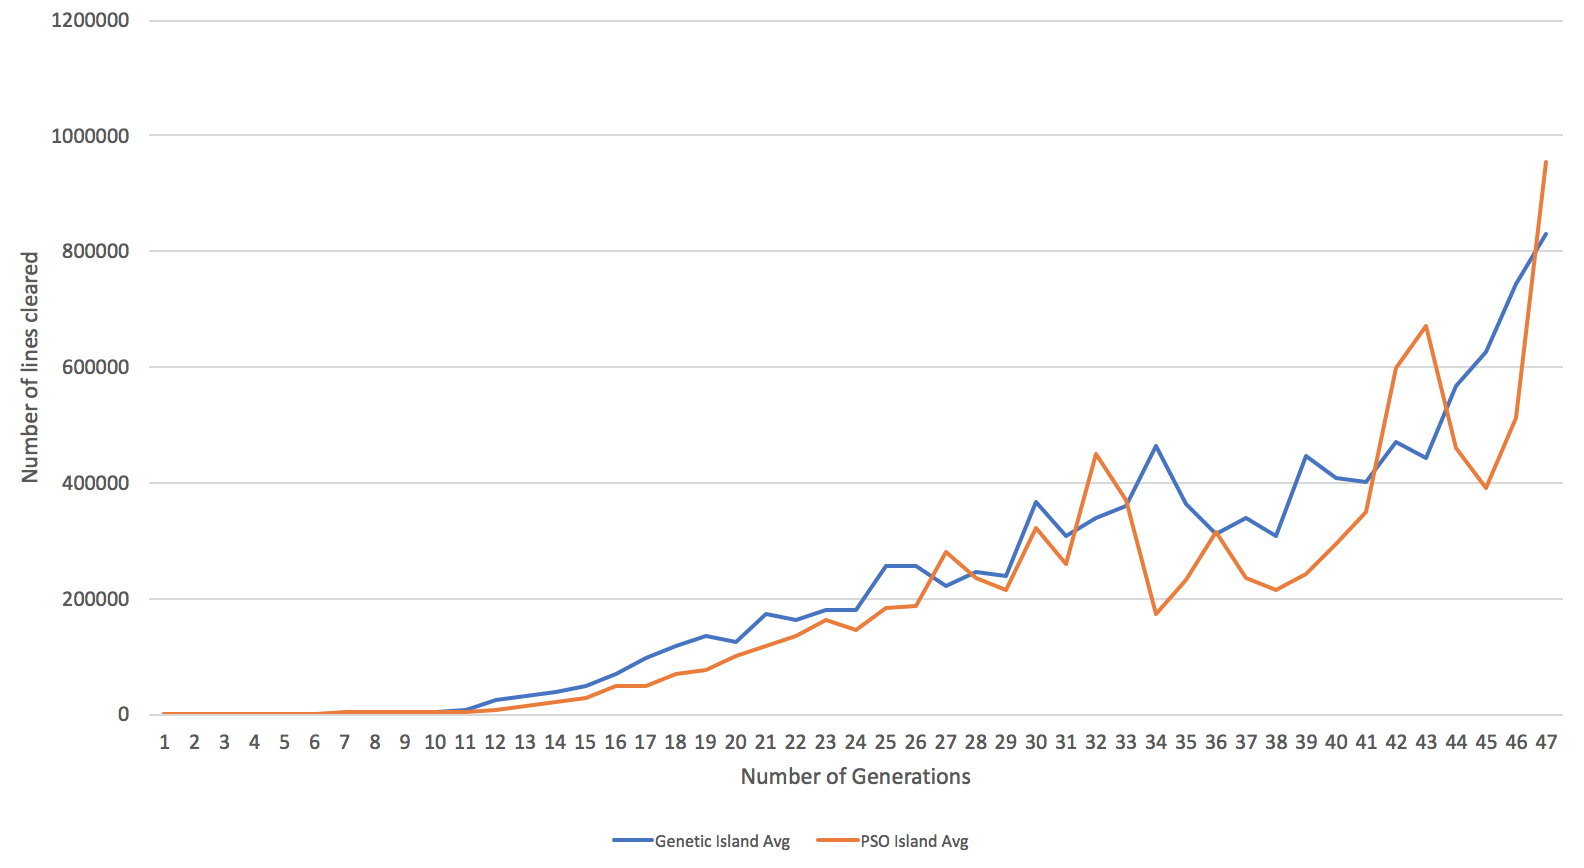
\includegraphics[scale=0.28]{learning/AlgoMax}
		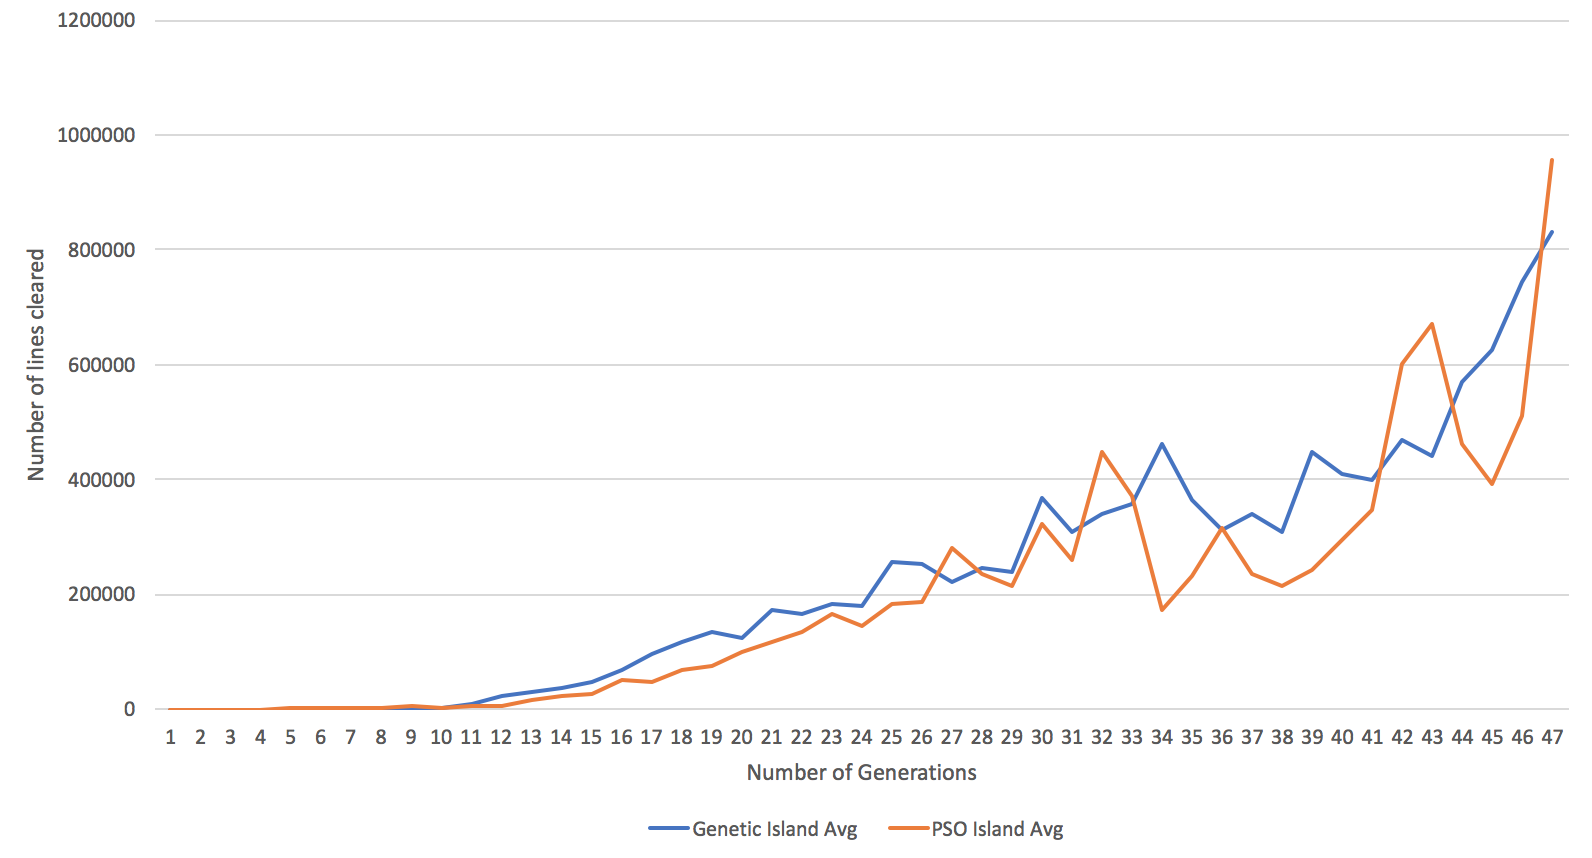
\includegraphics[scale=0.28]{learning/AlgoAvg}
		\centering
		\caption{Performance of the Learning Algorithm}
		\label{fig:learning}
	\end{figure}

	The first figure plots the lines cleared by the best heuristic in
	the GA and PSO islands over 47 generations, while the second figure plots
	the average lines cleared by the same populations. It can be seen that sometimes PSO leads the
	way in the first figure, producing a good heuristic that GA then builds
	upon. However, this is not always true, and in fact we did observe in other
	runs of the algorithm that sometimes GA also led the way.\\
	We also compared the results of our algorithm with Naive GA and Naive PSO
	(i.e. we ran them in isolation). The results obtained were:\\

	\begin{figure}[H]
		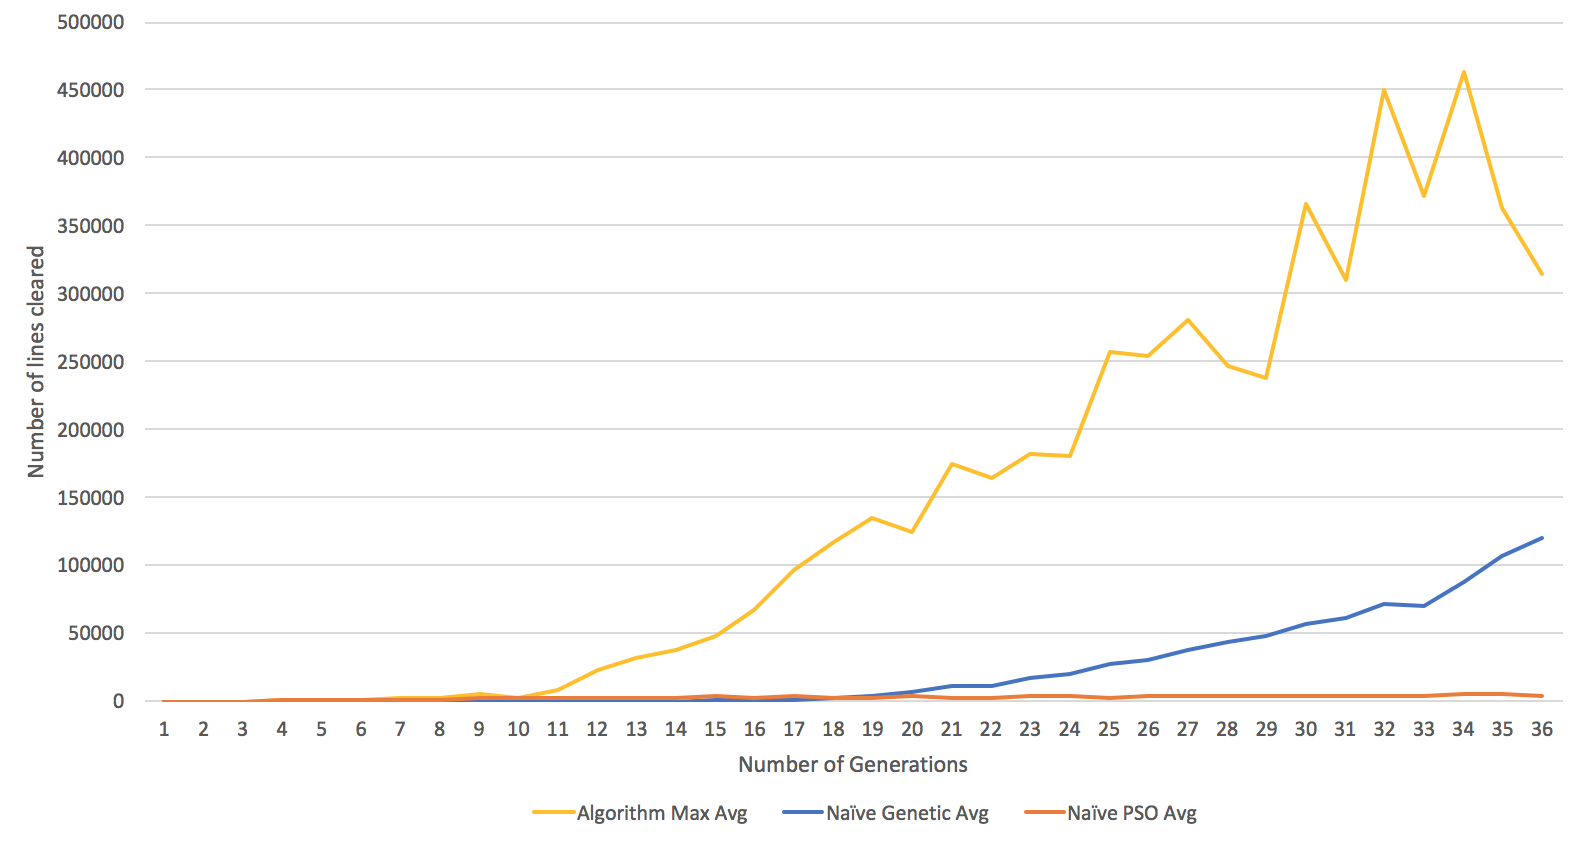
\includegraphics[scale=0.3]{learning/Naive}
		\centering
		\caption{Comparison of Learning Algorithm with Naive GA/PSO}
		\label{fig:naive}
	\end{figure}

	This figure plots the maximum of the average of GA and PSO islands for
	our learning algorithm, and compares it with the averages of Naive GA and
	Naive PSO. It can be seen that our algorithm performed far better, with PSO
	getting stuck at around 20 thousand lines cleared and GA rising very slowly.

	However, we can also observe from Figure \ref{fig:learning} that there is a large amount
	of variability in the results of the algorithm. One reason for this is the element
	of randomness in the algorithm itself, for example, in the mutation amount and threshold
	in GA and in the initial velocity imparted to a particle in PSO. There is
	a large amount of randomness in the game of tetris itself, as seen more clearly
	in the section below.

	Using a version of our algorithm that used 2 threads (one per island),
	we were able to get to a maximum of around 4 million lines cleared in
	around a day. Running a parallelised version (see below) we got to a maximum of
	around 18M in 10 hours.\\

	\textbf{Agent Performance}\\
	The best weights we obtained were:\\

	\vspace{-2mm}
	\begin{tabular}{ | c | c | c | c | c | c | c | c | c | c | c | c | c | }
		\hline
		$AltD$ & $ColT$ & $DW$ & $ColH$ & $CwH$ & $NHole$ & $NWell$ & $RC$ & $RowT$ & $TColH$ & $TColHD$ & $WB$ & $WellS$ \\ \hline
		0 & 0 & 0 & 0 & 0 & 0 & 0 & 0 & 0 & 0 & 0 & 0 & 0 \\ \hline
	\end{tabular}\\[0.25em]

	We ran the heuristic on \textbf{TODO} games, encapsulated in the following graph:\\

	% \begin{minipage}{0.4\linewith}
		\begin{figure}[h]
			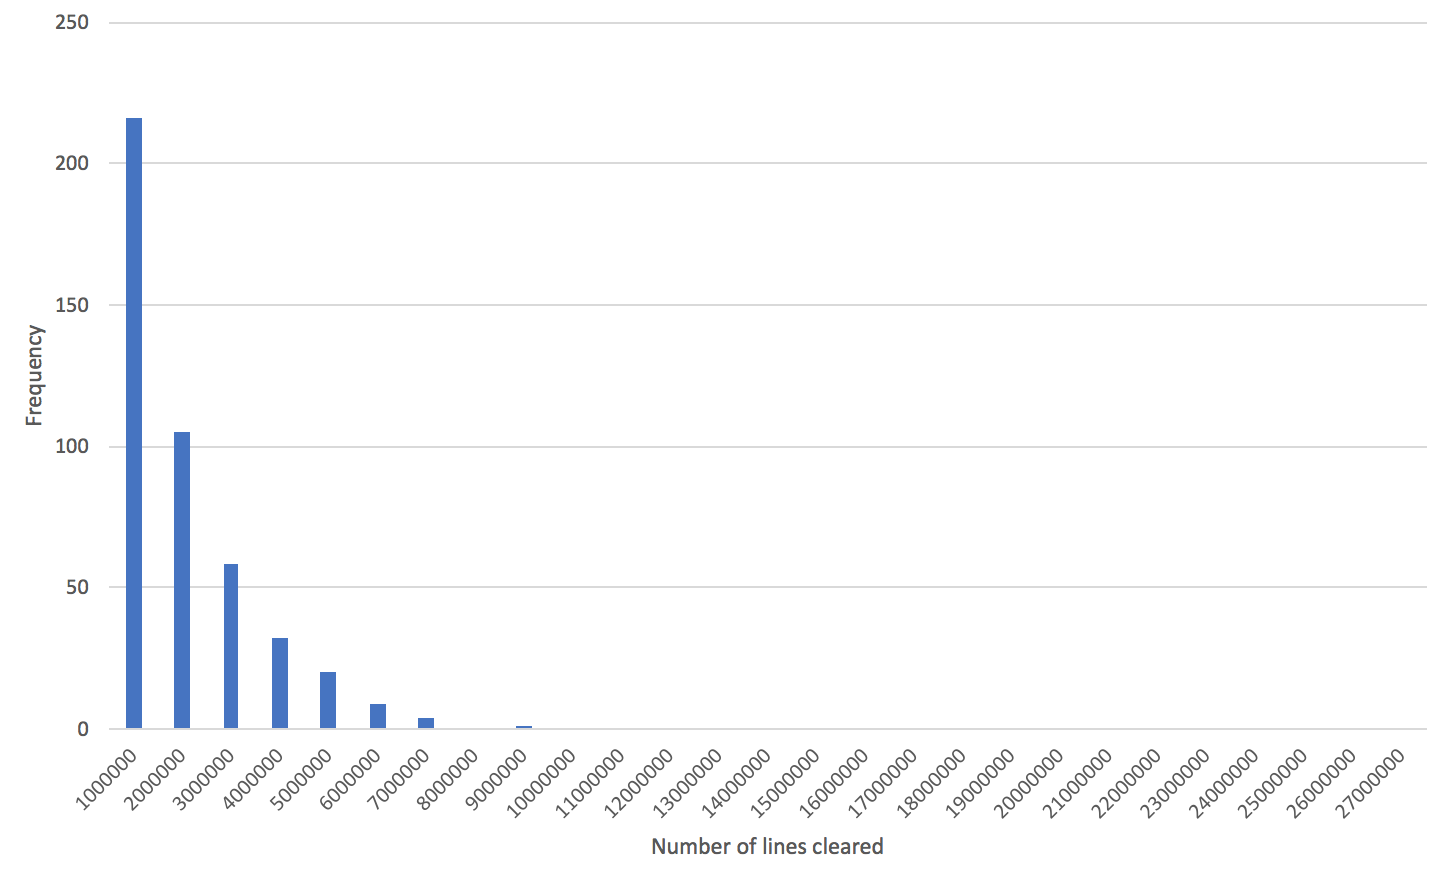
\includegraphics[scale=0.3]{heuristic/heuristic}
			\centering
			\caption{Performance of our Agent}
			\label{fig:agent}
		\end{figure}
	% \end{minipage}

	% \begin{minipage}{0.4\linewith}
		\begin{center}
			\begin{tabular}{ | c | c | c | }
				\hline
				Maximum & Minimum & Average \\ \hline
				0 & 0 & 0 \\ \hline
			\end{tabular}\\
		\end{center}
	% \end{minipage}




	As can be seen in Figure \ref{fig:agent}, there is a large variability in how
	well the heuristic performs, hitting a maximum of \textbf{TODO} and a minimum of \textbf{TODO}.
	This is likely because of the large randomisation within the game of tetris,
	with the sequences of pieces having a large impact on the performance.

	\vspace{-0.3cm}
    \section{Scaling to Big Data}
	\vspace{-0.3cm}
	In order to scale to Big Data, we considered how our algorithm performed in the presence
	of multiple cores. We found that parallelising our algorithms through the use
	of multithreading lead to a linear speedup, demonstrating that our algorithm scaled very
	well in the presence of multiple cores. We attribute this to the fact that
	both GA and PSO algorithms are embarassingly parallel, which
	is why we were able to achieve an optimal speedup quite easily.\\

	We parallelised our algorithm by running the PSO and GA islands on different cores,
	as well as by calculating the fitness of each population member on different cores.
	We did this as the major computational cost the algorithm was incurring came from
	the calculation of the fitness values, since that involved running entire tetris games. We started both algorithms as two separate jobs on single machines
	in the NSCC cluster (which provide 12 cores each) at the same time, and allowed them to run for around 20
	hours before comparing the results. We used the total number of lines cleared
	in the entire time span as a rough estimate of the total amount of
	CPU time used. Our results showed that the single-threaded algorithm cleared
	a total of $158182993$ lines, while the multi-threaded version cleared a total
	of $1899941699$ lines. This shows that parallelisation provides a speedup of 12 times,
	which is optimal since each machine has 12 cores.

	\vspace{-0.3cm}
    \section{Conclusion}
	To conclude, we believe that our agent is quite efficient, having managed to clear \textbf{TODO} lines.
	We have demonstrated that the use of GA and PSO, albeit with modifications such as
	information exchange and hyperparameter optimisation, can provide
	a reasonably effective learning algorithm. Our algorithm also scales very well the number
	of machines, thereby demonstrating that we can handle big data. While we believe that this
	idea can be taken further, and that with further optimisations, this algorithm can do even better,
	it suffices to say that we are quite satisfied with the results.


	\vspace{-0.3cm}
    \section{References}
	\bibliographystyle{apalike}
	\bibliography{./resources/bibliography/references}


\end{document}
